

\chapter{Supplementary data and figures Chapter 7}\raggedleft\textcolor{BLUEROYAL}{\LARGE{Why is selection for translationally optimal codons so scarce in metazoans?}}\\
\raggedleft\textcolor{BLUEROYAL}{\Large{Variation in fitness effects and drift intensity}}

{\hypersetup{linkcolor=GREYDARK}\minilof\newpage}

\graphicspath{{chap7-Translational Selection/figures/}}

\raggedright
\textbf{Estimating the strength of selection on synonymous codon usage using population genetics.}
\\
The frequency of optimal codons ($FOP$) reflects the balance between the optimal to non-optimal codons synonymous substitution rate ($K_{on}$) and the non-optimal to optimal codons synonymous substitution rate ($K_{no}$):

\[\text{Non-optimal codon } \autorightleftharpoons{$K_{no}$}{$K_{on}$} \text{ Optimal codon}\]

Substitution rates depend on the corresponding mutation rates ($\mu_{no}$, $\mu_{on}$) and fixation probabilities ($P_{no}$, $P_{on}$): \(K_{no} = 2\textit{N}_{\text{e}} \mu_{no} P_{no}\text{    and    }K_{on} = 2\textit{N}_{\text{e}} \mu_{on} P_{on}\), where \textit{N}$_{\text{e}}$ is the effective population size.

Fixation probabilities are given by:

\[P_{no} =  \frac{1 - e^{-4 \textit{N}_{\text{e}} f_0 s }}{1 - e^{-4 \textit{N}_{\text{e}} s }} = \frac{1 - e^{-2 s }}{1 - e^{-4 \textit{N}_{\text{e}} s }} \stackrel{\text{$s \rightarrow 0$}}{=} \frac{2 s }{1 - e^{-4 \textit{N}_{\text{e}} s }} \text{ similarly } P_{on} \stackrel{\text{$s \rightarrow 0$}}{=} \frac{-2 s }{1 - e^{4 \textit{N}_{\text{e}} s }}  \]


% \[\acrshort{K} = 2\acrshort{Ne}~\acrshort{mu}~P^F = 2\acrshort{Ne}~\acrshort{mu}~\frac{1 - e^{-4\acrshort{Ne}\acrshort{s} p}}{1 - e^{-4\acrshort{Ne}\acrshort{s}}} = 2\acrshort{Ne}~\acrshort{mu}~\frac{1 - e^{-2s}}{1 - e^{-4\acrshort{Ne}\acrshort{s}}}\]

Where $s$ is the selection coefficient in favor of optimal codons and $f_0$ the allele frequency of a new arrival mutation ($f_0 = 1/2\textit{N}_{\text{e}}$).

At equilibrium, the frequency of optimal codons is given by: \(FOP =  \frac{K_{no}}{K_{on} + K_{no}}\)

which can be written as:

\[FOP =  \frac{2 \textit{N}_{\text{e}} \mu_{no} P_{no}}{2 \textit{N}_{\text{e}} \mu_{no} P_{no}+2 \textit{N}_{\text{e}} \mu_{on} P_{on}}
=  \frac{\mu_{no} P_{no}}{\mu_{no} P_{no}+ \mu_{on} P_{on}} =  \frac{\frac{\mu_{no}}{\mu_{on}}  \frac{2s}{1 - e^{-4 \textit{N}_{\text{e}} s} }}{\frac{\mu_{no}}{\mu_{on}}  \frac{2s}{1 - e^{-4 \textit{N}_{\text{e}} s} } + \frac{-2s}{1 - e^{4 \textit{N}_{\text{e}} s} } }
\]

Let us note lambda, the ratio of mutation rates: $\lambda = \frac{\mu_{no}}{\mu_{on}}$

\[FOP =  \frac{\lambda}{\lambda + \frac{-(1 - e^{-4 \textit{N}_{\text{e}} s})}{1 - e^{4 \textit{N}_{\text{e}} s}}}
\]

\[\frac{1}{FOP} = 1 +   \frac{1}{\lambda} \times \frac{-(1 - e^{-4 \textit{N}_{\text{e}} s})}{1 - e^{4 \textit{N}_{\text{e}} s}}
\]

\[\frac{1}{FOP} - 1 =   \frac{-(1 - e^{-4 \textit{N}_{\text{e}} s})}{1 - e^{4 \textit{N}_{\text{e}} s}} \times \frac{1}{\lambda} 
\]

\[\frac{1-FOP}{FOP} \times \lambda = \frac{-(1 - e^{-4 \textit{N}_{\text{e}} s})}{1 - e^{4 \textit{N}_{\text{e}} s}} 
\]

\setcounter{equation}{0}
\begin{equation}
\frac{FOP}{1-FOP} \times \frac{1}{\lambda}  = \frac{1 - e^{4 \textit{N}_{\text{e}} s}}{-(1 - e^{-4 \textit{N}_{\text{e}} s})} 
\end{equation}

\newpage

With the following simplification:

\[ \frac{1 - e^{4 \textit{N}_{\text{e}} s}}{-(1 - e^{-4 \textit{N}_{\text{e}} s})} = \frac{1 - e^{4 \textit{N}_{\text{e}} s}}{-(1 - \frac{1}{e^{4 \textit{N}_{\text{e}} s}})} 
 = \frac{e^{4 \textit{N}_{\text{e}} s} \times (1-e^{4 \textit{N}_{\text{e}} s})}{1 - e^{4 \textit{N}_{\text{e}} s}} = e^{4 \textit{N}_{\text{e}} s}
\]

\[ (1) \rightarrow \frac{FOP}{1-FOP} \times \frac{1}{\lambda} = e^{4 \textit{N}_{\text{e}} s}
\]


Thus, the population-scaled selection coefficient ($S=4 \textit{N}_{\text{e}} s$) is given by:

\[ S = log(\frac{FOP}{1-FOP}) - log(\lambda) = logit(FOP) - log(\lambda)
\]

Hence, we expect a linear correlation between logit($FOP$) and $S$:

\[ logit(FOP) = S + log(\lambda)
\]


\setcounter{figure}{0}
\begin{figure*}[htbp]
    \centering                                                                            
    \includegraphics[width=0.8\textwidth]{Figure1_app.pdf}                                               
    \label{appfig:1}
\end{figure*}

\newpage

If for weakly-expressed genes there is no selection, implied by the non-variation of $FOP$ with gene expression, $S^{lx}\approx0$ :

\[ logit(FOP^{lx}) = 0 + log(\lambda)
\]


\[ logit(FOP^{hx}) = S^{hx} + log(\lambda)
\]

\[ S^{hx}  = logit(FOP^{hx}) - logit(FOP^{lx})
\]

\begin{figure*}[htbp]
    \centering                                                                            
    \includegraphics[width=\textwidth]{Figure2_app.pdf}                                               
    \label{appfig:2}
\end{figure*}


\newpage


\begin{figure*}[t]
    \centering                                                                            
    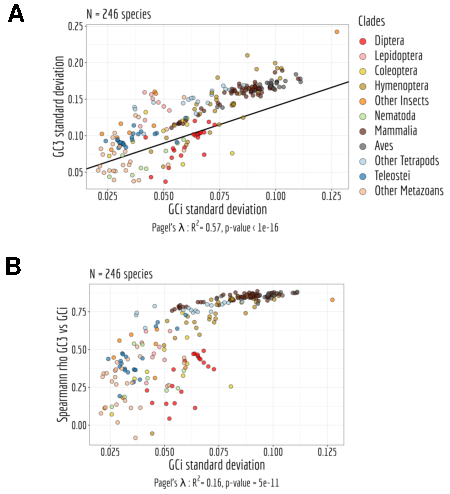
\includegraphics[width=0.6\textwidth]{Figure1_supp.pdf}                                               
    \caption[Intra-species codon usage variations]{\textbf{Intra-species codon usage variations.} \textbf{A}: Relationship between the standard deviation of the \textit{per} gene GC at the third position (GC3) and the GC in introns (GCi). \textbf{B}: Relationship between the Spearman coefficient (rho) reflecting the correlation between GC3 of genes and GC content in introns within a specific species, and the standard deviation of the \textit{per} gene GC in introns.}
    \label{suppfig:CU1}
\end{figure*}


\begin{figure*}[t]
    \centering                                                                            
    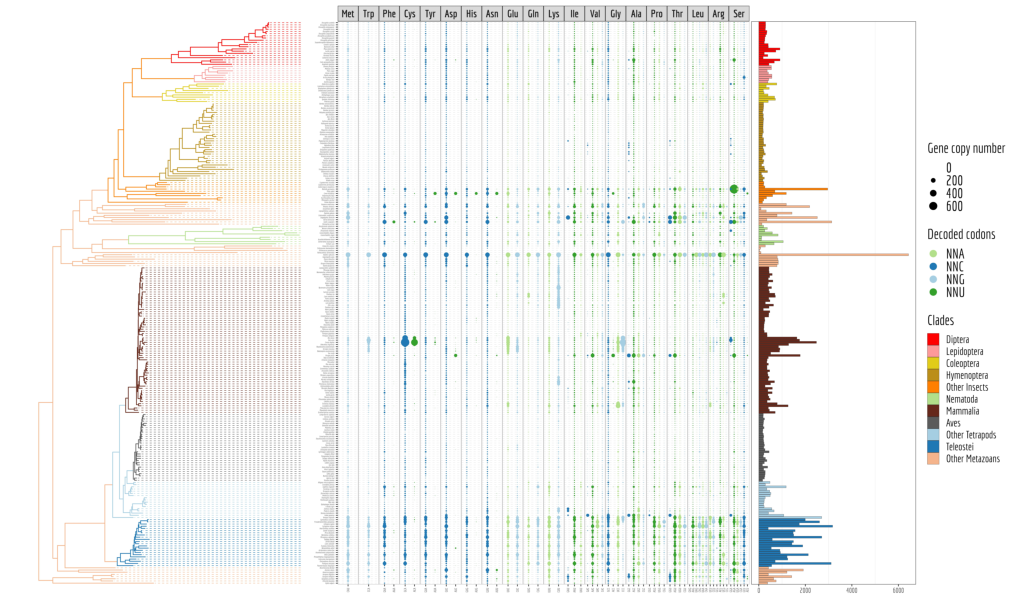
\includegraphics[width=\textwidth]{Figure2_supp.pdf}                                   
    \caption[tRNA gene copy number]{\textbf{tRNA gene copy number.} For the 257 studied species from left to right: phylogenetic tree, number of tRNA gene copy number \textit{per} amino acid \textit{per} codons and total number of tRNA gene copy.} 
    \label{suppfig:CU2}
\end{figure*}


\begin{figure*}[t]
    \centering                                                                            
    \includegraphics[width=\textwidth]{Figure3_supp.pdf}                                   
    \caption[tRNA abundance proxies]{\textbf{tRNA abundance proxies.} \textbf{A,B}: Relationship between the tRNA abundance measured by~\citet{behrens_high-resolution_2021} and the frequency of amino acid weighted by gene expression (FPKM). \textbf{C,D}: Relationship between tRNA gene copy number and the frequency of amino acid weighted by gene expression (FPKM). Left: \textit{Drosophila melanogaster}; Right: \textit{Homo sapiens}} 
    \label{suppfig:CU3}
\end{figure*}

\begin{figure*}[t]   
    \begin{center}                                                                       
        \includegraphics[width=\textwidth]{Figure5_supp.pdf}
    \end{center}                                                                       
    \caption[Counting for intronic background do not change the signal of translational selection]{\textbf{Counting for intronic background do not change the signal of translational selection.} The X-axis represents variations in POCs frequency, calculated as the difference between POC frequency in the 2\% most highly expressed genes and the 50\% least expressed genes. The Y-axis depicts the refined X-axis values by eliminating variations arising from non-adaptive processes, such as the difference in POC-control frequency between the 2\% most highly expressed genes and the 50\% least expressed genes. The black line represents the pagel's \textit{lambda} model, and the dotted line represents x=y.} 
    \label{suppfig:CU5}
\end{figure*}


\begin{figure*}[t]   
    \begin{center}                                                                       
        \includegraphics[width=\textwidth]{Figure6_supp.pdf}
    \end{center}                                                                       
    \caption[Non homogenous GC composition along genes]{\textbf{Non homogenous GC composition along genes.} \textbf{A,B}: Measured of the GC composition in introns using 100 bp windows from the start codon and the stop codon (kb, log scale). Equal group of genes have been formed regarding their length, represented by distinct color groups. \textbf{A}: \textit{Homo sapiens}; \textbf{B}: \textit{Drosophila melanogaster}} 
    \label{suppfig:CU6}
\end{figure*}


\begin{figure*}[t]
    \centering                                                                            
    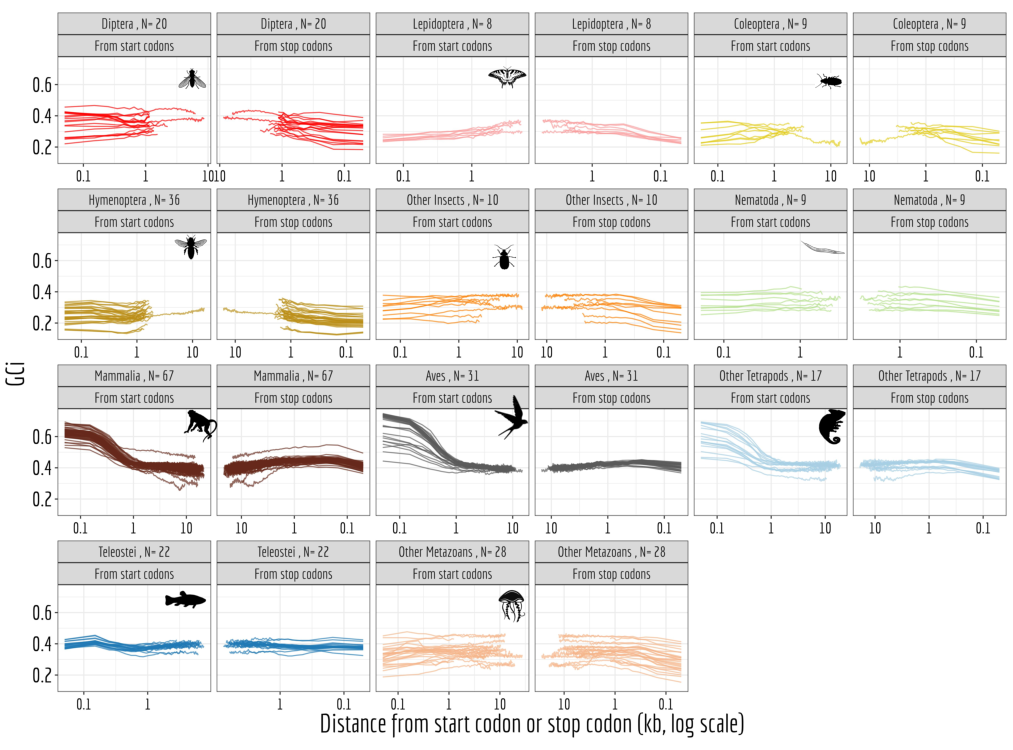
\includegraphics[width=\textwidth]{Figure7_supp.pdf}
    \caption[Non homogenous GC composition along genes for 11 clades]{\textbf{Non homogenous GC composition along genes for 11 clades.} Measured of the GC composition in introns using 100 bp windows from the start codon and the stop codon (kb, log scale). Each clade of the study is represented by color, one line represents one species.} 
    \label{suppfig:CU7}
\end{figure*}


\begin{figure*}[t]
    \centering                                                                            
    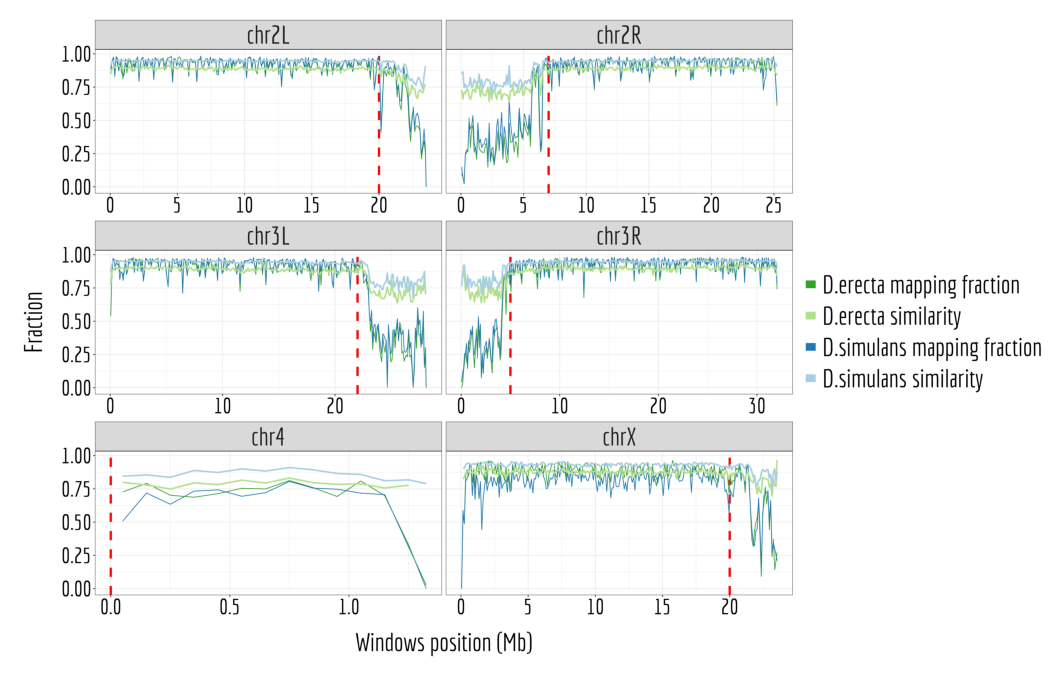
\includegraphics[width=\textwidth]{Figure8_supp.pdf}
    \caption[Multiple genome alignment quality of \textit{Drosophila simulans} and \textit{Drosophila erecta} on \textit{Drosophila melanogaster}]{\textbf{Multiple genome alignment quality of \textit{Drosophila simulans} and \textit{Drosophila erecta} on \textit{Drosophila melanogaster}.} 
    On the genome of \textit{Drosophila melanogaster} we quantify the fraction of sites mapped to the two other genomes, and the similarity of these sites. The red dotted lines represent the threshold above or below which the quality of the multiple genome alignment is poor.} 
    \label{suppfig:CU8}
\end{figure*}

\begin{figure*}[t]
    \centering                                                                            
    \includegraphics[width=\textwidth]{Figure9_supp.pdf}
    \caption[Differences in usage of putative-optimal codon between highly- and lowly-expressed genes in 6 species]{\textbf{Differences in usage of putative-optimal codon between highly- and lowly-expressed genes in 6 species.} Variation in the proportion of POC within coding sequences (POC1: dark blue; POC2: dark green) according to gene expression level. To control for variations in neutral substitution patterns, we analyzed the frequency of corresponding triplets within introns (POC1 control: light blue; POC2 control: light green). Each point represents a 2\% bin of genes, with the red point at the end of each POC1 curve denoting the 2\% most highly expressed genes. The red lines indicate the average POC1 proportions observed in the 50\% least expressed genes (FPKM, log scale).} 
    \label{suppfig:CU9}
\end{figure*}



\begin{figure*}[t]
    \centering                                                                            
    \includegraphics[width=\textwidth]{Figure10_supp.pdf}
    \caption[Relationship between \textit{N}$_{\text{e}}$ and its proxies]{\textbf{Relationship between \textit{N}$_{\text{e}}$ and its proxies.} Relationship between \textit{N}$_{\text{e}}$ and the longevity (days, log scale; \textbf{A}), body length (cm, log scale; \textbf{B}), body mass (kg, log scale; \textbf{C}), dN/dS (log scale; \textbf{D}). Pagel's \textit{lambda} model is used to take into account the phylogenetic structure of the data in a regression model (the regression line is displayed in black when the correlation is significant). } 
    \label{suppfig:CU10}
\end{figure*}
  

    
\begin{figure*}[t]
    \centering                                                                            
    \includegraphics[width=\textwidth]{Figure11_supp.pdf}
    \caption[Valine synonymous codons usage variations with expression among 4 species]{\textbf{Valine synonymous codons usage variations with expression among 4 species.} Relationship between the relative synonymous codon usage (RSCU) of valine synonymous codons (GTG/GTA/GTT/GTC) and gene expression in four species with different GC richness.} 
    \label{suppfig:CU11}
\end{figure*}


\begin{figure*}[t]
    \centering                                                                            
    \includegraphics[width=\textwidth]{Figure12_supp.pdf}
    \caption[Presence-Absence of tRNA defines set of putative-optimal codons for species subject to translational selection]{\textbf{Presence-Absence of tRNA defines set of putative-optimal codons for species subject to translational selection.} \textbf{A}: Illustration of the various possible pairings: Watson-Crick and wobble pairing. \textbf{B}: A boxplot illustrating the distribution of tRNA gene copy numbers across 26 species subject to translational selection (Lepidoptera and Diptera). The percentage of species lacking a tRNA gene copy is also indicated, highlighting the absence of tRNA isodecoder.} 
    \label{suppfig:CU12}
\end{figure*}
